\section{Implementação Concorrente}

\subsection{Implementação em Java}

\subsubsection{Descrição}

A estrutura geral do algoritmo é mantida em relação à versão serial: inicializar
centróides, iterar entre atribuição e recomputo, verificar convergência. O que muda
é \textit{como} os pontos são processados dentro de cada iteração.

Na versão serial, a thread principal lê cada ponto diretamente do arquivo, chama
\texttt{closestCentroid} e acumula os resultados em arrays compartilhados. Na versão
concorrente, a leitura ainda é feita sequencialmente, mas os pontos são agrupados em
lotes (\texttt{BATCH\_SIZE = 5.000}) e cada lote é submetido ao pool de workers como
uma tarefa independente. Os workers acumulam em arrays \emph{locais} e retornam um
\texttt{PartialResult}; a thread coordenadora reduz todos os parciais após coletar
os \texttt{Future}s.

Esse padrão --- \emph{dispatch em lotes, acumulação local, redução sequencial} ---
elimina a necessidade de sincronização nas regiões críticas CR1--CR4 sem uso de
\texttt{synchronized} ou variáveis atômicas. A chamada \texttt{Future.get()} garante
a relação happens-before entre a escrita dos workers e a leitura da coordenadora.

Uma cópia imutável dos centróides (\texttt{snapshot}) é tirada antes do dispatch de
cada iteração, garantindo que todos os workers vejam o mesmo estado de centróides
durante a iteração em andamento.

Foram implementadas três variantes concorrentes:

\begin{itemize}
    \item \textbf{v2-platform} --- pool fixo de $N$ platform threads para os workers
          e a thread \texttt{main} como coordenadora.
    \item \textbf{v2-virtual} --- pool fixo de $N$ virtual threads para os workers,
          mesma estrutura de v2-platform.
    \item \textbf{v2-hybrid} --- pool fixo de $N$ platform threads como workers
          CPU-bound e uma virtual thread como coordenadora
          (\texttt{newVirtualThreadPerTaskExecutor}). A virtual thread desmonta
          automaticamente durante \texttt{readLine} (I/O de disco) e durante cada
          \texttt{Future.get()} (park), liberando o carrier sem bloquear o
          \texttt{ForkJoinPool}.
\end{itemize}

As classes \texttt{CsvDataset}, \texttt{KMeansResult} e \texttt{Main} não foram
alteradas. As adições ficaram concentradas em \texttt{KMeans.java}:
dois records privados (\texttt{PartialResult}, \texttt{EvaluatePartial}) e três
métodos novos (\texttt{runClustering}, \texttt{processAssignBatch},
\texttt{processEvaluateBatch}). O método \texttt{evaluate} foi refatorado para
também usar o pool de workers. A classe \texttt{KMeansSampler} foi adicionada como
adaptador JMeter para os macrobenchmarks.

O diagrama de classes da Figura~\ref{fig:class-diagram-concurrent-java} mostra as
classes do projeto com as adições da versão concorrente em destaque.

\begin{figure}[H]
  \centering
  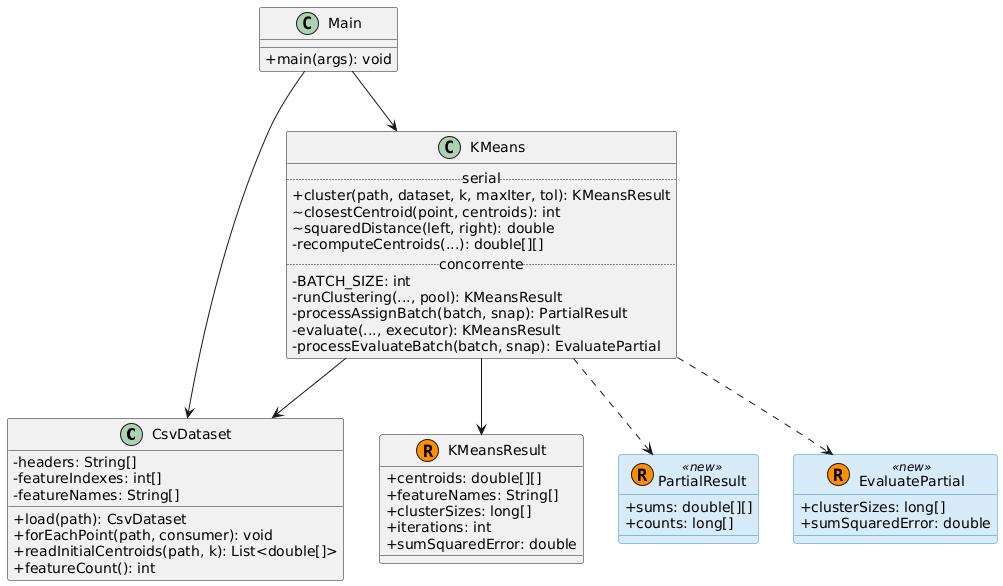
\includegraphics[width=0.85\textwidth]{img/4-concurrent/class-diagram}
  \caption{Diagrama de classes da implementação concorrente em Java. Elementos
           destacados são novos em relação à versão serial.}
  \label{fig:class-diagram-concurrent-java}
\end{figure}

A Figura~\ref{fig:snippet-concurrent-cluster} mostra a criação dos dois executores
e a submissão do método coordenador à virtual thread.

\begin{figure}[H]
  \centering
  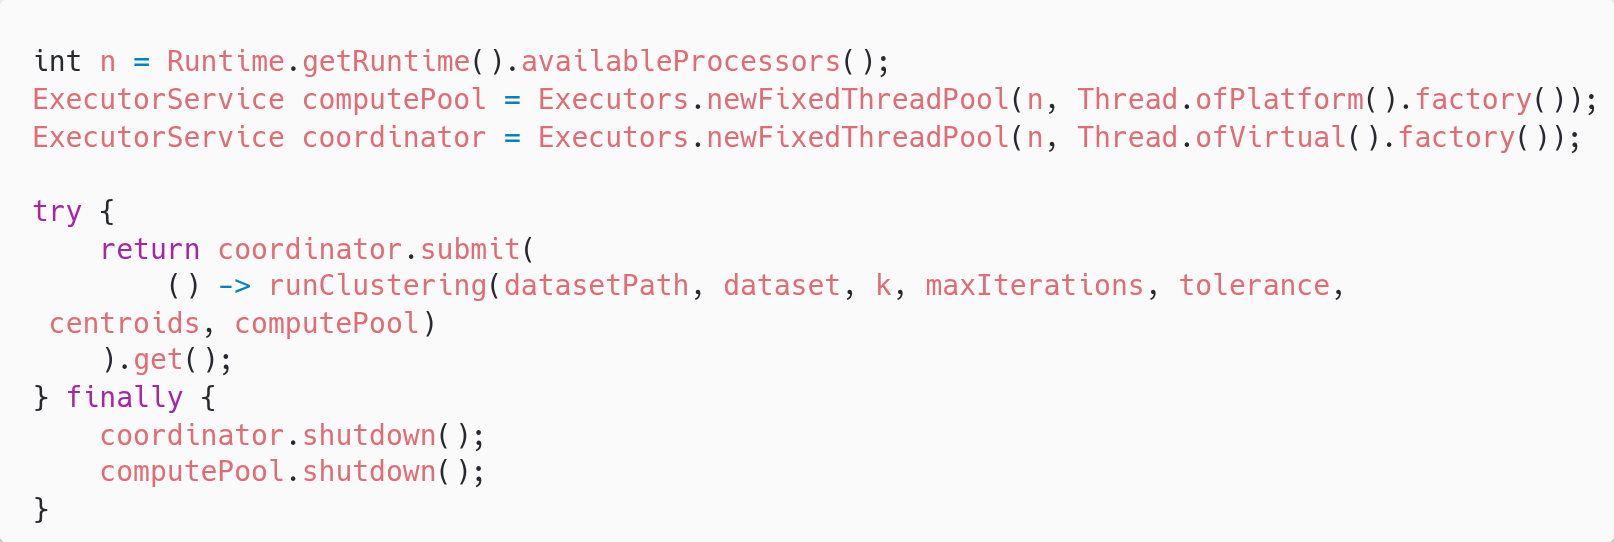
\includegraphics[width=0.85\textwidth]{img/4-concurrent/snippet-1}
  \caption{Criação dos executores e submissão do coordenador (\texttt{KMeans.cluster}).}
  \label{fig:snippet-concurrent-cluster}
\end{figure}

A Figura~\ref{fig:snippet-concurrent-dispatch} mostra o laço de dispatch de lotes
dentro de \texttt{runClustering}: a leitura sequencial acumula pontos até atingir
\texttt{BATCH\_SIZE}, quando cada lote é submetido ao pool e o buffer é esvaziado.

\begin{figure}[H]
  \centering
  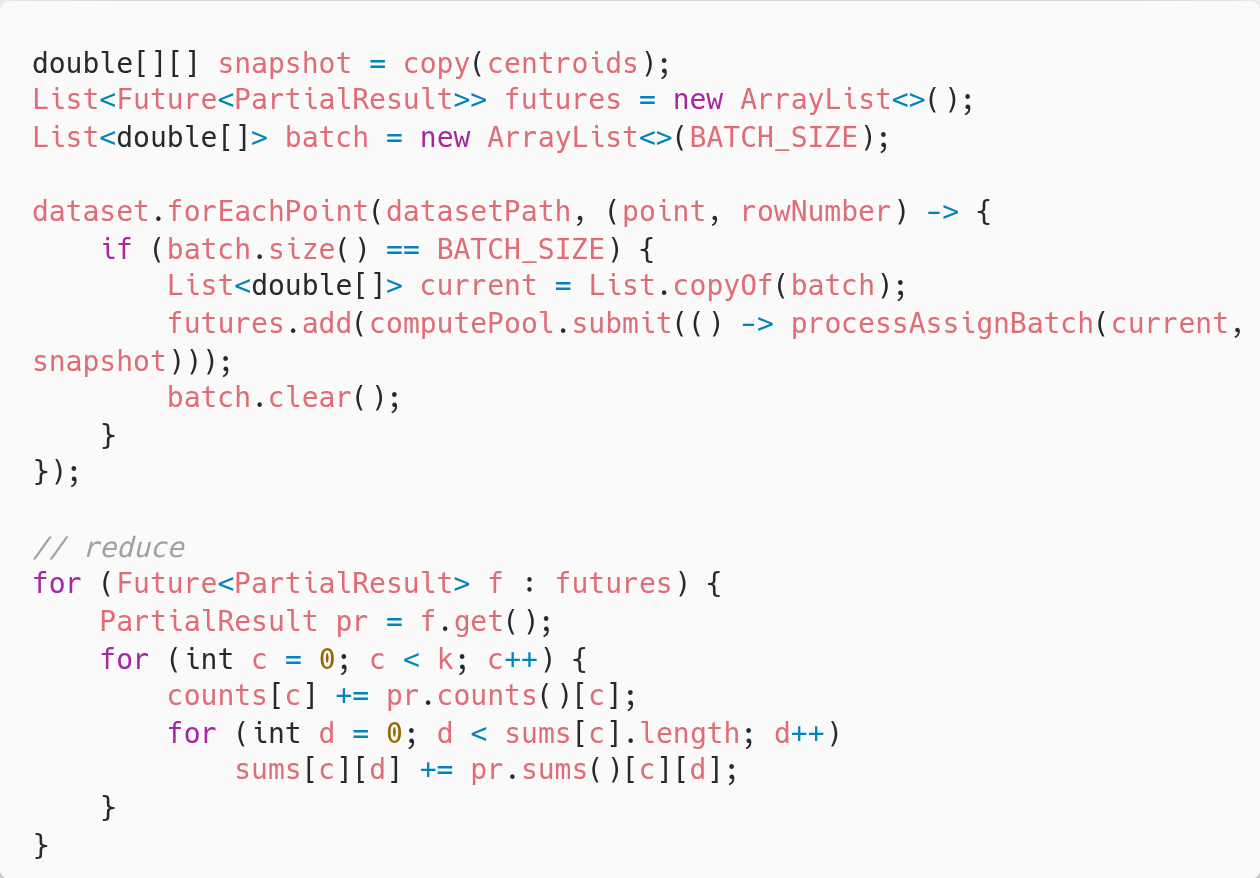
\includegraphics[width=0.85\textwidth]{img/4-concurrent/snippet-2}
  \caption{Dispatch de lotes e coleta de futures (\texttt{KMeans.runClustering}).}
  \label{fig:snippet-concurrent-dispatch}
\end{figure}

A Figura~\ref{fig:snippet-concurrent-batch} mostra \texttt{processAssignBatch}, o
método executado por cada worker: usa arrays locais (\texttt{localSums},
\texttt{localCounts}) sem compartilhamento, retornando um \texttt{PartialResult}
imutável.

\begin{figure}[H]
  \centering
  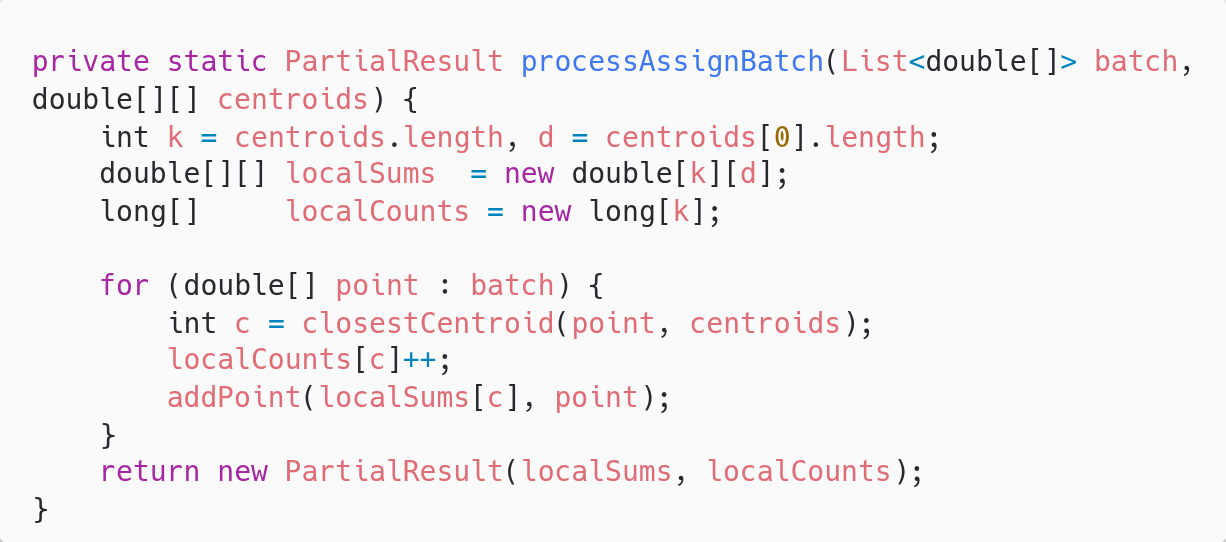
\includegraphics[width=0.85\textwidth]{img/4-concurrent/snippet-3}
  \caption{Processamento local de um lote sem arrays compartilhados
           (\texttt{KMeans.processAssignBatch}).}
  \label{fig:snippet-concurrent-batch}
\end{figure}

\subsubsection{Resultados}

\paragraph{Avaliação de Condição de Corrida}

Foram identificadas quatro regiões críticas na implementação concorrente, todas
relacionadas a acumulações que seriam problemáticas caso múltiplas threads
compartilhassem os mesmos arrays de escrita:

\begin{table}[H]
\centering
\begin{tabular}{llp{5.5cm}l}
\hline
\textbf{ID} & \textbf{Local} & \textbf{Operação} & \textbf{Risco} \\
\hline
CR1 & \texttt{processAssignBatch} & \texttt{counts[c]++}       & lost update em \texttt{long[]} \\
CR2 & \texttt{processAssignBatch} & \texttt{sums[c][d] += v}   & lost update em \texttt{double[][]} \\
CR3 & \texttt{processEvaluateBatch} & \texttt{sse += v}         & acumulação não atômica de double \\
CR4 & \texttt{processEvaluateBatch} & \texttt{clusterSizes[c]++} & lost update em \texttt{long[]} \\
\hline
\end{tabular}
\caption{Regiões críticas identificadas na implementação concorrente.}
\label{tab:critical-regions}
\end{table}

A Figura~\ref{fig:snippet-race-condition} mostra \texttt{processAssignBatch}, o
método executado por cada worker. As operações \texttt{localCounts[c]++} (CR1) e
\texttt{addPoint(localSums[c], point)} --- que internamente faz \texttt{sums[c][d] += v}
(CR2) --- seriam race conditions se os arrays fossem compartilhados entre workers.
A implementação usa arrays \emph{locais} por tarefa, tornando-as thread-safe.

\begin{figure}[H]
    \centering
    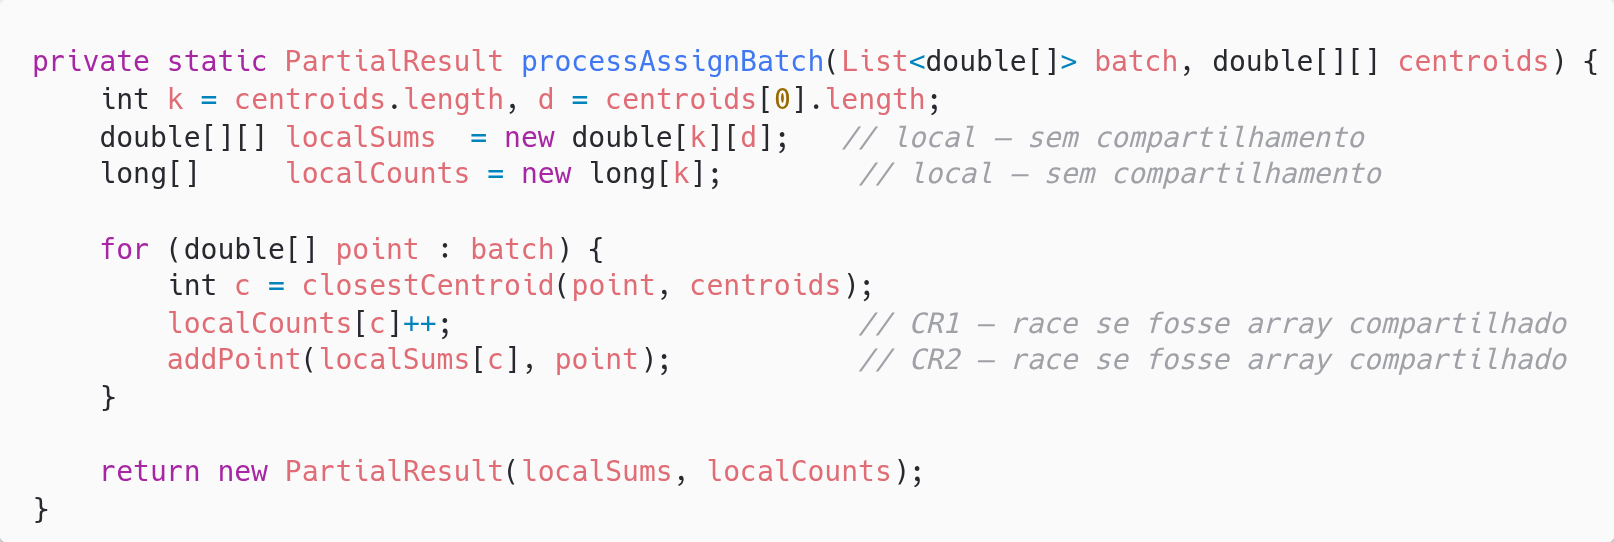
\includegraphics[width=0.85\textwidth]{img/4-concurrent/snippet-race-condition}
    \caption{Operações CR1 e CR2 em \texttt{processAssignBatch}: \texttt{localCounts[c]++}
             e \texttt{addPoint} seriam race conditions se os arrays fossem compartilhados.}
    \label{fig:snippet-race-condition}
\end{figure}

Os testes foram executados com JCStress 0.16, preset \texttt{default}, 6 forks por
teste e 5 iterações de 1.000 ms por fork. A
Tabela~\ref{tab:jcstress-results} apresenta o resultado consolidado.

\begin{table}[H]
\centering
\begin{tabular}{llll}
\hline
\textbf{ID} & \textbf{Resultado} & \textbf{Outcome FORBIDDEN} & \textbf{Freq.\ máx.} \\
\hline
JCS1 & \textbf{PASSOU}            & nenhum                   & ---      \\
JCS2 & \textbf{PASSOU}            & nenhum                   & ---      \\
JCS3 & FALHOU (esperado) & \texttt{"1"} lost update em \texttt{counts[0]++}  & 28,31\% \\
JCS4 & FALHOU (esperado) & \texttt{"1.0"} lost update em \texttt{sums[0]+=1.0} & 27,10\% \\
\hline
\end{tabular}
\caption{Resultados JCStress --- regiões críticas da implementação concorrente.}
\label{tab:jcstress-results}
\end{table}

JCS1 e JCS2 não produziram nenhum outcome FORBIDDEN: a leitura concorrente é segura.
JCS3 e JCS4 falharam como esperado: lost updates ocorrem em até 28\% das amostras
com compilação C2 e em 0,01\% com o Interpreter.

\paragraph{Avaliação com Microbenchmark}

Os microbenchmarks foram executados com JMH 1.37 sobre JDK 25.0.1 (OpenJDK 64-Bit
Server VM), com 1 fork, 1 iteração de aquecimento de 10 s e 3 iterações de medição
de 10 s cada. O dataset utilizado é o mesmo da versão serial ($\approx$1 GB).

\subparagraph{v2-platform --- Platform Threads.}
Pool fixo de $N$ threads de plataforma criado com
\texttt{Executors.newFixedThreadPool(N,~Thread.ofPlatform().factory())},
onde $N$ é o número de processadores lógicos disponíveis. A thread principal lê o
CSV em lotes de 5.000 pontos e submete cada lote ao pool imediatamente, de modo
que os workers processam em paralelo enquanto a leitura continua.

\begin{table}[h]
\centering
\begin{tabular}{llrrrr}
\hline
\textbf{ID} & \textbf{Benchmark} & \textbf{Serial} & \textbf{v2-platform} & \textbf{Erro ($\pm$)} & \textbf{Unidade} \\
\hline
B1 & Execução completa (\textit{k}=10, maxIter=20) & 212{,}57 & 214{,}87 & 29{,}10 & s/op \\
B2 & Custo por iteração (\textit{k}=10, maxIter=5) &  60{,}05 &  60{,}69 &  6{,}41 & s/op \\
B3 & \texttt{closestCentroid} (\textit{k}=10, 38 dims) &  96{,}82 & 102{,}24 &  3{,}92 & ns/op \\
B4 & \texttt{squaredDistance} (38 dims)               &   9{,}31 &   9{,}70 &  2{,}71 & ns/op \\
\hline
\end{tabular}
\caption{Resultados JMH --- serial vs.\ v2-platform.}
\label{tab:jmh-v2-platform}
\end{table}

B1 e B2 são equivalentes ao serial (diferença $< 1{,}5\%$). O parsing CSV
sequencial na thread principal continua dominando o tempo de execução. B3 e B4
permanecem na mesma faixa.

\subparagraph{v2-virtual --- Virtual Threads.}
Pool fixo de $N$ virtual threads criado com
\texttt{Executors.newFixedThreadPool(N,~Thread.ofVirtual().factory())},
onde $N$ é o número de processadores lógicos disponíveis --- estrutura
idêntica à de v2-platform, alterando apenas a fábrica de threads. Cada virtual
thread é escalonada pelo JVM sobre carriers de um \texttt{ForkJoinPool} interno,
sem corresponder a uma thread de SO.

\begin{table}[h]
\centering
\begin{tabular}{llrrrr}
\hline
\textbf{ID} & \textbf{Benchmark} & \textbf{Serial} & \textbf{v2-virtual} & \textbf{Erro ($\pm$)} & \textbf{Unidade} \\
\hline
B1 & Execução completa (\textit{k}=10, maxIter=20) & 212{,}57 & 211{,}64 & 260{,}68 & s/op \\
B2 & Custo por iteração (\textit{k}=10, maxIter=5) &  60{,}05 &  71{,}61 & 227{,}05 & s/op \\
B3 & \texttt{closestCentroid} (\textit{k}=10, 38 dims) &  96{,}82 & 101{,}11 &   8{,}06 & ns/op \\
B4 & \texttt{squaredDistance} (38 dims)               &   9{,}31 &   9{,}58 &   1{,}23 & ns/op \\
\hline
\end{tabular}
\caption{Resultados JMH --- serial vs.\ v2-virtual.}
\label{tab:jmh-v2-virtual}
\end{table}

B1 (211,64 s) é equivalente ao serial, mas com margem de erro elevada ($\pm$260 s).
B2 também apresenta alta variância ($\pm$227 s), reflexo da imprevisibilidade do
\texttt{ForkJoinPool} para tarefas CPU-bound que nunca bloqueiam. B3 e B4
permanecem na mesma faixa.

\subparagraph{v2-hybrid --- Abordagem Híbrida.}
Dois executores separados: um \texttt{computePool} de $N$ platform threads
(\texttt{Thread.ofPlatform().factory()}) para os workers CPU-bound, e um
\texttt{coordinator} com \texttt{Executors.newVirtualThreadPerTaskExecutor()}
que executa \texttt{runClustering()} em uma única virtual thread. O coordenador
desmonta durante a leitura do CSV (\texttt{readLine}) e durante cada
\texttt{Future.get()}, liberando o carrier enquanto aguarda os workers.

\begin{table}[h]
\centering
\begin{tabular}{llrrrr}
\hline
\textbf{ID} & \textbf{Benchmark} & \textbf{Serial} & \textbf{v2-hybrid} & \textbf{Erro ($\pm$)} & \textbf{Unidade} \\
\hline
B1 & Execução completa (\textit{k}=10, maxIter=20) & 212{,}57 & 215{,}69 & 59{,}78 & s/op \\
B2 & Custo por iteração (\textit{k}=10, maxIter=5) &  60{,}05 &  60{,}44 &  5{,}33 & s/op \\
B3 & \texttt{closestCentroid} (\textit{k}=10, 38 dims) &  96{,}82 & 102{,}07 & 26{,}17 & ns/op \\
B4 & \texttt{squaredDistance} (38 dims)               &   9{,}31 &   9{,}87 &  1{,}14 & ns/op \\
\hline
\end{tabular}
\caption{Resultados JMH --- serial vs.\ v2-hybrid.}
\label{tab:jmh-v2-hybrid}
\end{table}

B1 (215,69 s) é equivalente ao serial, com margem de erro moderada ($\pm$59,78 s):
os workers de plataforma estabilizam o escalonamento, mas o coordenador virtual
adiciona alguma variabilidade ao bloquear em \texttt{Future.get()}. B2 ($\pm$5,33 s)
é estável. B3 e B4 permanecem na mesma faixa.

\paragraph{Avaliação com Macrobenchmark}

Os macrobenchmarks foram executados com JMeter 5.6.3 sobre JDK 25.0.1, com
$k = 10$, \texttt{maxIter} = 3 e \texttt{tol} = 0{,}0. Cada configuração
(GC $\times$ threads) rodou por 120 s com ramp-up de 30 s.

\subparagraph{v2-platform --- Platform Threads.}
A Tabela~\ref{tab:jmeter-v2-platform} apresenta o throughput (execuções/min)
por número de threads JMeter e coletor de GC.

\begin{table}[H]
\centering
\begin{tabular}{rrrrr}
\hline
\textbf{Threads} & \textbf{G1GC} & \textbf{ZGC} & \textbf{ParallelGC} & \textbf{Unidade} \\
\hline
1  & 1{,}65 & 1{,}42 & 1{,}59 & execuções/min \\
2  & 1{,}95 & 1{,}96 & 2{,}11 & execuções/min \\
4  & 3{,}92 & 2{,}42 & 2{,}62 & execuções/min \\
8  & 3{,}08 & 2{,}45 & 2{,}79 & execuções/min \\
16 & 4{,}49 & 4{,}10 & 4{,}39 & execuções/min \\
\hline
\end{tabular}
\caption{Throughput por número de threads e coletor de GC --- v2-platform.}
\label{tab:jmeter-v2-platform}
\end{table}

Com 1 thread JMeter, o throughput é $\approx$1,6 exec/min. O ganho não é linear
com mais threads: cada execução cria internamente $N$ workers, de modo que
8 threads JMeter geram até $8 \times N$ workers competindo por CPU e I/O de disco.

\subparagraph{v2-virtual --- Virtual Threads.}
A Tabela~\ref{tab:jmeter-v2-virtual} apresenta o throughput (execuções/min)
por número de threads JMeter e coletor de GC.

\begin{table}[H]
\centering
\begin{tabular}{rrrrr}
\hline
\textbf{Threads} & \textbf{G1GC} & \textbf{ZGC} & \textbf{ParallelGC} & \textbf{Unidade} \\
\hline
1  & 1{,}59 & 1{,}55 & 1{,}62 & execuções/min \\
2  & 2{,}17 & 1{,}99 & 2{,}13 & execuções/min \\
4  & 3{,}29 & 3{,}02 & 2{,}14 & execuções/min \\
8  & 4{,}00 & 2{,}75 & 3{,}77 & execuções/min \\
16 & 4{,}55 & 4{,}09 & 4{,}34 & execuções/min \\
\hline
\end{tabular}
\caption{Throughput por número de threads e coletor de GC --- v2-virtual.}
\label{tab:jmeter-v2-virtual}
\end{table}

Com 1 thread JMeter, o throughput é $\approx$1,6 exec/min. Com 4 threads G1GC
chega a 3,29 exec/min; com 8 threads a 4,00 exec/min. Em 16 threads, todas as
configurações de GC convergem para $\approx$4,3--4,6 exec/min.

\subparagraph{v2-hybrid --- Abordagem Híbrida.}
A Tabela~\ref{tab:jmeter-v2-hybrid} apresenta o throughput (execuções/min)
por número de threads JMeter e coletor de GC.

\begin{table}[H]
\centering
\begin{tabular}{rrrrr}
\hline
\textbf{Threads} & \textbf{G1GC} & \textbf{ZGC} & \textbf{ParallelGC} & \textbf{Unidade} \\
\hline
1  & 1{,}60 & 1{,}45 & 1{,}59 & execuções/min \\
2  & 2{,}13 & 1{,}98 & 2{,}14 & execuções/min \\
4  & 2{,}67 & 2{,}51 & 2{,}71 & execuções/min \\
8  & 3{,}44 & 3{,}21 & 3{,}38 & execuções/min \\
16 & 4{,}53 & 4{,}09 & 4{,}40 & execuções/min \\
\hline
\end{tabular}
\caption{Throughput por número de threads e coletor de GC --- v2-hybrid.}
\label{tab:jmeter-v2-hybrid}
\end{table}

Com 1 thread JMeter, o throughput é $\approx$1,6 exec/min. Com 8 threads G1GC
chega a 3,44 exec/min; com 16 threads a 4,53 exec/min. O ZGC fica levemente
abaixo das demais configurações em todos os níveis.

\paragraph{Avaliação de Profile}

O profile foi capturado com JFR (\texttt{settings=profile}) sobre uma execução
completa do algoritmo ($k=10$, \texttt{maxIter=3}, G1GC, dataset $\approx$1 GB).
A gravação durou $\approx$113 s e foi analisada com a ferramenta \texttt{jfr}
do JDK 25.

\subparagraph{v2-platform --- Platform Threads.}

\textbf{Hot Methods.}
Foram coletadas 12.157 amostras de CPU no total. A
Tabela~\ref{tab:jfr-hot-v2-platform} mostra os métodos mais frequentes.

\begin{table}[H]
\centering
\begin{tabular}{lrl}
\hline
\textbf{Método} & \textbf{CPU (\%)} & \textbf{Categoria} \\
\hline
\texttt{FloatingDecimal.parseDouble}           & 86{,}6 (main) & Parsing CSV \\
\texttt{FloatingDecimal.readJavaFormatString}  & --- & Parsing CSV \\
\texttt{String.split}                          & --- & Parsing CSV \\
\texttt{BufferedReader.readLine}               & --- & I/O \\
\texttt{KMeans.closestCentroid}                & 13{,}4 (workers) & Algoritmo \\
\texttt{KMeans.squaredDistance}                & --- & Algoritmo \\
\hline
\end{tabular}
\caption{Hot methods na implementação v2-platform (JFR, 12.157 amostras).}
\label{tab:jfr-hot-v2-platform}
\end{table}

A thread \texttt{main} concentra 10.521 amostras (86,6\%), com parsing CSV
dominando. Os 16 workers de plataforma somam 1.636 amostras (13,4\%),
com \texttt{closestCentroid} e \texttt{squaredDistance} no topo.

\textbf{GC.}
Foram realizadas 1.005 coletas Young GC em 113 s (8,9/s), com pausa total de
1.006 ms (0,89\%). O heap oscila entre $\approx$5 MB e $\approx$250 MB. O GC não é um gargalo.

\textbf{Threads.}
O peak foi de 24 threads ativas: 1 \texttt{main}, 16 workers de plataforma e
7 threads internas da JVM (GC, JIT, JFR).

\textbf{Síntese.}
O parsing CSV domina o CPU na thread \texttt{main} (86,6\%). Os workers
executam o cálculo aritmético em paralelo (13,4\%).

\subparagraph{v2-virtual --- Virtual Threads.}

\textbf{Hot Methods.}
Foram coletadas 10.164 amostras de CPU no total. A
Tabela~\ref{tab:jfr-hot-v2-virtual} mostra os métodos mais frequentes.

\begin{table}[H]
\centering
\begin{tabular}{lrl}
\hline
\textbf{Método} & \textbf{CPU (\%)} & \textbf{Categoria} \\
\hline
\texttt{String.split}                          & 99{,}8 (main) & Parsing CSV \\
\texttt{FloatingDecimal.copyDigits}            & --- & Parsing CSV \\
\texttt{FloatingDecimal.readJavaFormatString}  & --- & Parsing CSV \\
\texttt{BufferedReader.readLine}               & --- & I/O \\
\texttt{KMeans.closestCentroid}                & 0{,}2 (workers) & Algoritmo \\
\hline
\end{tabular}
\caption{Hot methods na implementação v2-virtual (JFR, 10.164 amostras).}
\label{tab:jfr-hot-v2-virtual}
\end{table}

A thread \texttt{main} concentra 10.143 amostras (99,8\%). Apenas 21 amostras
foram capturadas em workers --- todas no carrier \texttt{ForkJoinPool-1-worker-1}.
Os demais carriers não aparecem porque cada lote termina em menos de 10 ms
(intervalo de amostragem do JFR). O parsing CSV domina o CPU.

\textbf{GC.}
Foram realizadas 1.148 coletas Young GC em 109 s (10,5/s), com pausa total de
955 ms (0,88\%). O GC não constitui gargalo.

\textbf{Threads.}
O peak foi de 10 threads ativas: 1 \texttt{main}, carriers do \texttt{ForkJoinPool}
(raramente visíveis ao JFR) e threads internas da JVM.

\textbf{Síntese.}
O parsing CSV domina o CPU (99,8\%). As tarefas de lote são CPU-bound e de
curta duração, não chegando a acionar o mecanismo de unmount das virtual threads.

\subparagraph{v2-hybrid --- Abordagem Híbrida.}

\textbf{Hot Methods.}
Foram coletadas 2.133 amostras de CPU no total. A
Tabela~\ref{tab:jfr-hot-v2-hybrid} mostra os métodos mais frequentes.

\begin{table}[H]
\centering
\begin{tabular}{lrl}
\hline
\textbf{Método} & \textbf{CPU (\%)} & \textbf{Categoria} \\
\hline
\texttt{KMeans.squaredDistance}  & 83{,}4 (workers)    & Algoritmo \\
\texttt{KMeans.closestCentroid}  & 14{,}2 (workers)    & Algoritmo \\
\texttt{KMeans.addPoint}         &  1{,}5 (workers)    & Algoritmo \\
coordenador virtual              &  0{,}1              & Coordenação \\
\hline
\end{tabular}
\caption{Hot methods na implementação v2-hybrid (JFR, 2.133 amostras).}
\label{tab:jfr-hot-v2-hybrid}
\end{table}

Os workers de plataforma concentram 2.130 amostras (99,9\%), com
\texttt{squaredDistance} (83,4\%) e \texttt{closestCentroid} (14,2\%) no topo.
O coordenador virtual aparece em apenas 3 amostras (0,1\%): durante
\texttt{readLine} e \texttt{Future.get()}, a virtual thread desmonta e libera
o carrier, tornando-se invisível ao JFR.

\textbf{GC.}
Foram realizadas 1.072 coletas Young GC em 140 s (7,7/s), com pausa total de
1.178 ms (0,84\%). O GC não constitui gargalo.

\textbf{Threads.}
O peak foi de 28 threads ativas: 1 \texttt{main}, 1 virtual thread coordenadora,
16 workers de plataforma e $\approx$10 threads internas da JVM.

\textbf{Síntese.}
O parsing CSV desaparece do perfil de CPU: o coordenador virtual desmonta
durante \texttt{readLine}, e o profiler captura apenas o trabalho aritmético
dos workers.

\iffalse % ============================================================
% ERLANG — seção desativada, manter para uso futuro
\subsection{\sout{Implementação em Erlang}}

\subsubsection{\sout{Descrição}}

\subsubsection{\sout{Resultados}}

\paragraph{\sout{Avaliação de Condição de Corrida}}

\paragraph{\sout{Avaliação com Microbenchmark}}

\paragraph{\sout{Avaliação com Macrobenchmark}}

\paragraph{\sout{Avaliação de Profile}}
\fi % ============================================================

\subsection{Discussão}

\textbf{Condições de corrida.}
Os testes JCStress identificaram quatro regiões críticas (CR1--CR4), todas
associadas a acumulações em arrays compartilhados. JCS3 e JCS4 confirmaram
lost updates em até 28\% das amostras quando a sincronização é omitida. A
solução adotada --- acumulação local por worker com redução após
\texttt{Future.get()} --- elimina a race condition sem uso de
\texttt{synchronized} ou atomics.

\textbf{Comparação de abordagens --- microbenchmark.}
A Tabela~\ref{tab:jmh-comparativo} compara as três variantes com a versão serial.

\begin{table}[H]
\centering
\begin{tabular}{lrrrr}
\hline
\textbf{Abordagem} & \textbf{B1 (s/op)} & \textbf{B2 (s/op)} & \textbf{Erro B1} & \textbf{Erro B2} \\
\hline
Serial      & 212{,}57 & 60{,}05 &  $\pm$34{,}48 &  $\pm$2{,}46 \\
v2-platform & 214{,}87 & 60{,}69 &  $\pm$29{,}10 &  $\pm$6{,}41 \\
v2-virtual  & 211{,}64 & 71{,}61 & $\pm$260{,}68 & $\pm$227{,}05 \\
v2-hybrid   & 215{,}69 & 60{,}44 &  $\pm$59{,}78 &  $\pm$5{,}33 \\
\hline
\end{tabular}
\caption{Comparativo JMH entre abordagens (s/op).}
\label{tab:jmh-comparativo}
\end{table}

Nenhuma abordagem reduz o tempo médio em relação ao serial: o parsing CSV
sequencial é o gargalo comum a todas. v2-virtual apresenta variância muito
alta ($\pm$260 s em B1), reflexo do \texttt{ForkJoinPool} ao lidar com tarefas
CPU-bound. v2-platform e v2-hybrid têm variância próxima ao serial.

\textbf{Comparação de abordagens --- macrobenchmark.}
A Tabela~\ref{tab:jmeter-comparativo} compara o throughput (G1GC) por número
de threads JMeter.

\begin{table}[H]
\centering
\begin{tabular}{lrrrrr}
\hline
\textbf{Abordagem} & \textbf{1 t} & \textbf{2 t} & \textbf{4 t} & \textbf{8 t} & \textbf{16 t} \\
\hline
v2-platform & 1{,}65 & 1{,}95 & 3{,}92 & 3{,}08 & 4{,}49 \\
v2-virtual  & 1{,}59 & 2{,}17 & 3{,}29 & 4{,}00 & 4{,}55 \\
v2-hybrid   & 1{,}60 & 2{,}13 & 2{,}67 & 3{,}44 & 4{,}53 \\
\hline
\end{tabular}
\caption{Throughput (execuções/min, G1GC) por abordagem e número de threads JMeter.}
\label{tab:jmeter-comparativo}
\end{table}

Com poucos threads JMeter (1--2), as três variantes são equivalentes. Com 4
threads, v2-platform tem o maior throughput (3,92 exec/min). Com 8 threads,
v2-virtual supera as demais (4,00 exec/min): seus workers são virtual threads
multiplexadas sobre $N$ carriers, evitando a saturação do escalonador de kernel
que ocorre com $8 \times N$ platform threads reais. Em 16 threads, todas
convergem para $\approx$4,5 exec/min.

\textbf{Comparação de coletores de GC.}
O GC tem impacto pequeno em todas as variantes (pausas $< 1\%$ do tempo total).
O ZGC fica levemente abaixo de G1GC e ParallelGC em configurações com muitas
threads simultâneas, pelo custo das barreiras de escrita do seu algoritmo.
G1GC e ParallelGC têm desempenho semelhante entre si.
